% Introduction
% story line:
% multi-modal long-document conditioned video generation
% motivation:
% manually create video for research present is labor-intensive
% much demand for explanatory videos to amplify research impact
% challenge
% no benchmark and metric
% ?

% [teaser]
% 1. reflect present video (paper input + slide + sub + talking head + cursor)
% 2. 
\vspace{-1\baselineskip} 
\section{Introduction}
\vspace{-0.3\baselineskip} 
% [impact background] improtance of academic presentation video creation, how larbor-intensive it is. --> automatic presentation video generation is improtant and practially usefull.
% [compared with existing method] agent for sub-task, natural video gen
% [what we did] benchmark, p2vagent, evalution


% ##[impact background] automatic  presentation video is labor-intensive important for academic communication, but it is labor-intensive including slide creation, talking head per slide / recording, subtitling;
% average spend a hour to develop a 5-10mins. 
% ##[compared with existing method] Despite there has some work for auto PPT, poster, coding but automatically presentation video generation being a promising direction and less exploration.
% compare with natural video gen, presentation video is unique because
% 1. sourced from long-context paper (interleaved, multi-page, professional), information compression;
% 2. it pair with multiple aligned channel / multi-tasks: slide creation , text2speech, subtitling, talking head, cursor. project-level
% 3. lack of evaluation and metric. what define a good presentation video, considering the knowledge conveying via visual format, audio-friendly; 
% In this work, we focus on this problem, particualry, we address two core problems:
% 1. how to automatically create a presentation video from paper;
% for this 
% Paper2Video
% A:
% B:

% 2. how to evaluate a presentation video.
% for this, 
% PaperTalk-101
Academic presentation videos are widely used in research communication, serving as a crucial and effective means to bridge researchers, as many conferences require them as an essential material for submission. However, the manual creation of such a video is highly labor-intensive, requiring slide design, subtitle writing, per-slide recording, and careful editing, which on average may take several hours to produce a $2$ to $10$ minute video for a scientific paper. Despite some prior works on slide and poster generation~\cite{sun2021d2s,zheng2025pptagent,pang2025paper2poster} and other AI4Research tasks~\cite{ai4research,writing_ass,goldsack2022making,paper2code,paper2agent}, automatic academic presentation video generation is a superproblem of them, a practical yet more challenging direction. 

 % such as Veo3~\cite{deepmind2025veo3}, 
 \vspace{-0.2\baselineskip} 
Unlike natural video generation~\cite{sd_video,show_1,wan,deepmind2025veo3}, presentation video exhibits distinctive characteristics, including multi-sensory integration, multi-figure conditioning, and high text density, which highlight the limitations of current natural video generation models~\cite{ma2025controllable}. Specifically, academic presentation video generation faces several crucial challenges:
\textit{a.} It originates from long-context papers that contain dense text as well as multiple figures and tables;
\textit{b.} It requires the coordination of multiple aligned channels, including slide generation~\cite{zheng2025pptagent}, subtitling, text-to-speech~\cite{tts-f5}, cursor control, and talking head generation~\cite{fantasytalking,cui2024hallo2};
\textit{c.} It lacks well-defined evaluation metrics: what constitutes a good presentation video, particularly in terms of knowledge conveyance and audience accessibility. Even for the state-of-the-art end-to-end video–audio generation model Veo3~\cite{deepmind2025veo3}, notable limitations remain in video length, clarity of dense on-screen text, and multi-modal long-document condition.
In this work, we try to solve these two core problems as shown in Figure~\ref{fig:teaser}.
%{\textbf{(i)} What defines a good academic presentation video}, and {\textbf{(ii)} How to effectively automatically generate such a video from a research paper}.

\vspace{-0.2\baselineskip} 
To enable comprehensive evaluation of academic presentation video generation, we present the \textbf{\bench} Benchmark, comprising $101$ paired research papers and author-recorded presentation videos from recent conferences, together with original slides and speaker identity metadata. Based on this benchmark, we develop a suite of metrics to comprehensively evaluate generation quality from multiple dimensions: 
\textbf{(i)} Meta Similarity — We employ a VLM to evaluate the alignment of generated slides and subtitles with human-designed counterparts.
\textbf{(ii)} PresentArena — We use a VideoLLM as a proxy audience to perform double-order pairwise comparisons between generated and human-made videos.
Notably, the primary purpose of a presentation is to \textit{effectively convey the information contained in the paper}. To this end, we introduce \textbf{(iii) PresentQuiz}, which treats the VideoLLMs as the audience and requires them to answer paper-derived questions given the videos. Furthermore, another important purpose of presentation video is to \textit{enhance the visibility and impact of the author’s work}. Motivated by real-conference interactions, we introduce \textbf{(iv) IP Memory}, which measures how well an audience can associate authors and works after watching presentation videos.

% \textbf{(iii) Academic IP} — Inspired by real conference scenarios, this metric examines whether, after watching a video, researchers can recall the work and formulate relevant questions, thereby measuring how memorable and academically impactful the presentation video is.

\begin{figure}[!t]  % h=here, t=top, b=bottom, p=单独浮动页,!=放宽限制
    \vspace{-1\baselineskip}
    \centering
    \small
    \captionsetup{skip=2pt}  
    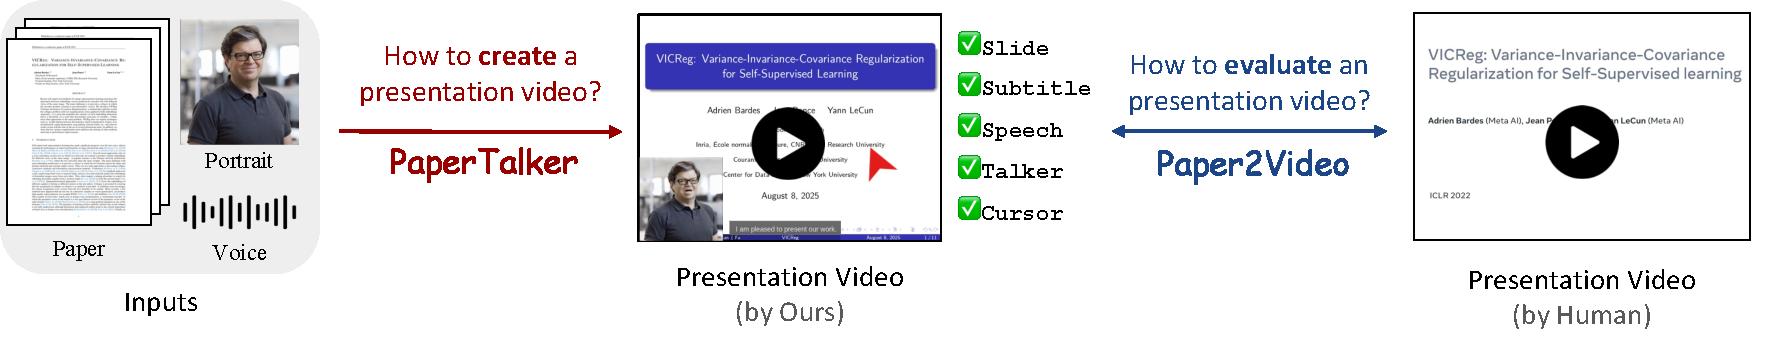
\includegraphics[width=\linewidth]{figure/teaser.pdf}
    \caption{{This work solves two core problems for academic presentations:} \textbf{Left:} \textit{how to create a presentation video from a paper?} {\agent} -- an agent integrates slide, subtitling, cursor grounding, speech synthesis, and talking-head video rendering. \textbf{Right:} \textit{how to evaluate a presentation video?} {\bench} -- a benchmark with well-designed metrics to evaluate presentation quality.}
    \label{fig:teaser}
    \vspace{-0.5\baselineskip}
\end{figure}

% \kevin{here, quite long, need to have (i) (ii) (iii) to structure the process;}
\vspace{-0.2\baselineskip} 
To effectively generate ready-to-use academic presentation videos, we propose \textbf{\agent}, the first multi-agent framework that enables academic presentation video generation from research papers and speaker identity. It integrates subsequent key modules: \textbf{(i)} Slide Generation. Instead of adopting the commonly used format (\textit{e.g.}, pptx, XML) from a template slide as in ~\cite{zheng2025pptagent}, we employ LaTeX code for slide generation from sketch, given its formal suitability for academic use and higher efficiency. Specifically, we employ a state-of-the-art Coder to generate code and introduce an effective \textbf{focused debugging} strategy, which iteratively narrows the scope and resolves compilation errors using feedback that indicates the relevant rows.
%\kevin{effective \textbf{debugging} strategy}. 
To address the insensitivity of LLMs to fine-grained numerical adjustments, we propose a novel method called \textbf{Tree Search Visual Choice}. This approach systematically explores parameter variations to generate multiple branches, which are then concatenated into a single figure. A VLM is then tasked with selecting the optimal branch, thereby effectively improving element layouts such as figure and font size.
\textbf{(ii)} Subtitling and Cursor Grounding. We generate subtitles and cursor prompts for each sentence based on the slides. Then we achieve cursor spatial-temporal alignment using \textbf{Computer-use grounding model}~\cite{lin2025showui, qin2025ui} models and WhisperX~\cite{bain2023whisperx} respectively. \textbf{(iii)} Speech Synthesis and Talking-head Rendering. We synthesize personalized speech via text-to-speech models~\cite{chen2024f5} and produce talking-head videos~\cite{cui2024hallo2,fantasytalking} for author presentations. Inspired by human recording practice and the independence between each slide, we \textbf{parallelize generation} across slides, achieving a speedup of more than $\mathbf{6\times}$.
% \kevin{comment camel} Our multi-agent framework is implemented within the \texttt{CAMEL}\footnote{https://github.com/camel-ai/camel},  promoting simplicity and enabling scalability. 
We will open-source all our data and codebase to empower the research community.

\vspace{-0.4\baselineskip} 
To summarize, our contributions are as follows:
\vspace{-0.6\baselineskip} 
\begin{itemize}[leftmargin=*]
    \item We present \bench, the first high-quality benchmark of $101$ papers with author-recorded presentation videos, slides, and speaker metadata, together with evaluation metrics: Meta Similarity, PresentArena, PresentQuiz, and IP Memory.
    
    \vspace{-0.2\baselineskip} 
    \item We propose {\agent}, the first multi-agent framework for academic presentation video generation. It introduces three key modules: \textbf{(i)} tree search visual choice for fine-grained slide generation; \textbf{(ii)} a GUI-grounding model coupled with WhisperX for spatial-temporal aligned cursor grounding; and \textbf{(iii)} slide-wise parallel generation to improve efficiency.

    
    % \kevin{include a/b/c/d}, key insights such as visual mcts; leverage cua / whisperx for spatial-temporal-grounded alignment; to speedup, parallel 
    % the first multi-agent framework for academic presentation video generation, featuring unified multi-channel integration, CoT-based slide debugging with visual inspection, and parallel video synthesis for efficiency.

    \vspace{-0.2\baselineskip} 
    \item Results on {\bench} confirm the effectiveness of {\agent}, which outperforms human-made presentations by 10\% in PresentQuiz accuracy and achieves comparable ratings in user studies, indicating that its quality approaches that of human-created content.
    
    % which achieves \textbf{more than 10\% higher} PresentArena score, PresentQuiz accuracy, and IP Memory than top-performing baselines such as Veo3. [comparable with human-made]
    % PresentArena score & human study - [comparable with human-made] 
  
    
    % \kevin{add details number regarding our optimization and improvement here\kevin{sota video-audio gen like veo3 demonstrate significant limitation (xx\%). meanwhile, our agent beat veo3, how sim. to human, other multi-agent }}
\end{itemize}





% to summary, our contributions are:
% 1. Benchmark
% % 1
% 2. For effective, agent core design -- module A: debug from code, enable it effectively debugging with visual inspection
% 3. For effecient, we design a parallel generation -- module B, which speedup the heavy talking head generation with \%x, 

% % 2
% 2. we propose Paper2Video agent, it is the first multi-agent workflow, which integrate XXX tools work together, enable automatically without human;
% 3. To enhance coding-rich visual task, we develop a better debugging strategy,

% 4. Expes demonstratate, metric, 